\section{The OCR Process}

A brief of the character recognition process and the hardships that one may face during it. A description of the characters utilized can also be given here.

\subsection{Equations}

The minor equations or definitions of variables can be inserted directly in the paragraph line, for example, consider that you want to define a story $\vect{h}_i^n = w_{i-1}. w_{i-2}, \dots, w_{i-n+1}$ associated with a $w_i$ symbol. Note that a simple way to ensure uniformity in the style of the equations is to write the mathematical formulations always in the corresponding environment, that is, using \verb!$a + b$! to write for example $a + b$ (do not write directly as the text a + b). On the other hand, remember that the units of measurement should always be written in \emph{round} format, so that they are not mistaken by variables (for example, $1\,\text{m} = 100\,\text{cm}$ instead of $1m = 100cm$).

\subsection{Figures}

Figures should be properly referenced using the traditional \LaTeX\ commands, and should never be placed as loose elements within the text. The figure caption is automatically placed using the environment
\begin{verbatim}
\begin{figure}[!tb]
  \centering
  \includegraphics[<options>]{<file>}
  \caption{Epigraph} \label{<label>}
\end{figure}
\end{verbatim}
and filling in the corresponding field in \verb!\caption{<>}! (see Fig.~\ref{fig-1}). The figures can be contained in PDF, JPG or PNG files, among others. Within the field \verb![<options>]! you can use the \verb![width=.8\columnwidth]! if it is necessary to adjust the size of the figure. Fig 1 has been set as an example using the factor \verb!.8! .

\begin{figure}[!tb] 
 \centering
 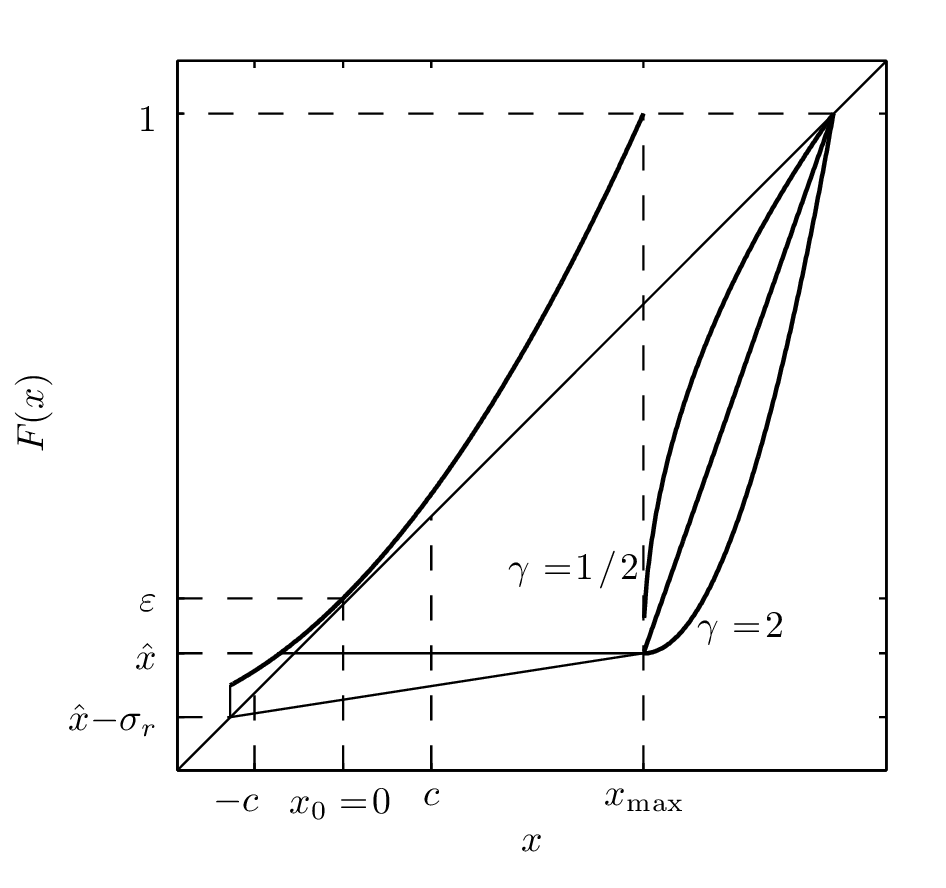
\includegraphics[width=.8\columnwidth]{figura1} 
 \caption{Outline of the map used indicating the different ways of reinjection and the effect of noise.} \label{fig-1}
\end{figure}

Preferably, the figures should be arranged at the beginning or end of a column of text (for which the \texttt{[!tb]} option is used), and in general it is not advisable to arrange the figures on special pages at the end ??from work??. Do not include additional breaks or spaces at the ends of the figures as these are duly defined in the class file. If Cartesian axes are used in the figure, always remember to describe what each axis (labels) corresponds to, with a font of size no smaller than 7 pt for easy reading. To refer to a figure, use the abbreviated form Fig. followed by the \verb!\ref{label}! command, except when it is at the beginning of a paragraph, in which case the whole word should be used.

% \begin{figure*}[!tb] 
%  \centering
%  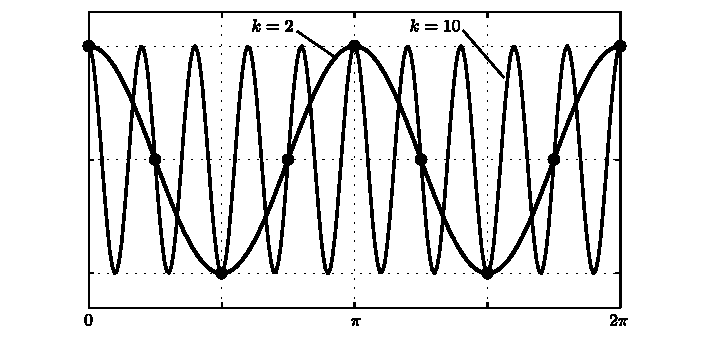
\includegraphics{figura2.pdf} 
%  \caption{Example of the aliasing that occurs in a grid with $N = 8$ nodes. Both modes ($k = 2$ and $k = 10$) take the same values at the grid points.} \label{fig-2}
% \end{figure*}

\begin{table}[!b]
 \centering
  \caption{Final results and relative error reduction (averages over 10 training and test partitions).} \label{table-1}
 {\small
 \begin{tabular}{ccccc}
  \hline
  \hline
  \thead{Recognition \\ Errors} & \thead{SER \\ \%} & \thead{WER \\ \%} & \thead{WAER \\ \%} &
                        \thead{Reduction \\ \% WER} \\
  \hline
  \hline
  Reference & $38.30$ & $7.54$ & $8.53$ & $-$ \\
  \hline
  HMM-PASS & $30.55$ & $5.36$ & $6.67$ & $28.91$ \\
  1-PASS & $25.50$ & $4.76$ & $5.70$ & $36.87$   \\
  \hline
  \hline
 \end{tabular}}
\end{table}

\subsection{Bibliographic citations}

\begin{itemize}
 \item Book: Authors, year in parentheses. Title in italics, editorial, place of publication \cite{Alarcos1999}. It is included using the \texttt{@book} option in the references file.
%
 \item Book chapter: Authors, year in parentheses. Chapter title in quotes. In: book title in italics of the book, pages, editorial, place of publication \cite{Mitchell2001}. It is included with the \texttt{@inbook} field in the reference file.
%
 \item Article in periodic magazine: Authors, year in parentheses. Title of the article in quotation marks, name of the magazine in italics, volume, number in parentheses, pages \cite{ArslanHansen1996, WangEtAl2015}. It is included using the \texttt{@article} option.
%
 \item Conferences: Authors, year in parentheses. Article title in quotes. In: title of the memoirs or of the event in italics, editorial of the publication of the memoirs, place of publication, pages \cite{BarkovaJouvet1999}. It is included with the \texttt{@inproceedings} field in the reference file.
%
 \item Website: Authors, year in parentheses. Title of the article in quotes, taken from <URL>, query date of the web page in parentheses \cite{CFDwebpage}. It is included with the \texttt{@webpage} option.
%
 \item Technical report: Authors, year in brackets. Title of the report in quotes, ``Report Nº'', institution in italics, place of publication \cite{NACA460}. It is included using the \texttt{@techreport} field.
%
 \item Thesis, thesis or final work: Authors, year in parentheses. Title in italics, type of work. Institution, place of presentation \cite{Krause2014}. It is included using the \texttt{@thesis} field in the reference file.
%
 \item Manual or technical report: Authors, year in parentheses. Title in italics, organization or institution, place of publication \cite{Indura2010}. It is included with the \texttt{@manual} option.
%
 \item Other forms of communication: to reference other forms of communication, you must always specify the author or entity, the year and the way in which the communication was made. You can optionally include a title and an explanatory note. These types of references are included using the \texttt{@other} field.
\end{itemize}

The bibliographic references section is labeled as ``References'' (or with its equivalent depending on the chosen language) and has a particular style for the paragraph, where the indentation is eliminated and the font size is reduced (fixed at 8 pt ). References should be showed in alphabetical order taking into account the last name of the first author, regardless of the order of appearance in the text. Remember that all references included in the bibliography section must be duly cited in the text.

To fully satisfy the definitions established for the bibliography and facilitate subsequent editing and publishing tasks, it is strongly recommended to use the reference style provided, including bibliography by the command
\begin{verbatim}
 \insertbibliography{<file.bib>} 
\end{verbatim}
at the end of manuscript.